% Options for packages loaded elsewhere
\PassOptionsToPackage{unicode}{hyperref}
\PassOptionsToPackage{hyphens}{url}
%
\documentclass[
  11pt,
]{article}
\usepackage{lmodern}
\usepackage{amssymb,amsmath}
\usepackage{ifxetex,ifluatex}
\ifnum 0\ifxetex 1\fi\ifluatex 1\fi=0 % if pdftex
  \usepackage[T1]{fontenc}
  \usepackage[utf8]{inputenc}
  \usepackage{textcomp} % provide euro and other symbols
\else % if luatex or xetex
  \usepackage{unicode-math}
  \defaultfontfeatures{Scale=MatchLowercase}
  \defaultfontfeatures[\rmfamily]{Ligatures=TeX,Scale=1}
\fi
% Use upquote if available, for straight quotes in verbatim environments
\IfFileExists{upquote.sty}{\usepackage{upquote}}{}
\IfFileExists{microtype.sty}{% use microtype if available
  \usepackage[]{microtype}
  \UseMicrotypeSet[protrusion]{basicmath} % disable protrusion for tt fonts
}{}
\makeatletter
\@ifundefined{KOMAClassName}{% if non-KOMA class
  \IfFileExists{parskip.sty}{%
    \usepackage{parskip}
  }{% else
    \setlength{\parindent}{0pt}
    \setlength{\parskip}{6pt plus 2pt minus 1pt}}
}{% if KOMA class
  \KOMAoptions{parskip=half}}
\makeatother
\usepackage{xcolor}
\IfFileExists{xurl.sty}{\usepackage{xurl}}{} % add URL line breaks if available
\IfFileExists{bookmark.sty}{\usepackage{bookmark}}{\usepackage{hyperref}}
\hypersetup{
  pdftitle={Promise and peril: Agnostic identification methods for detecting differential item functioning},
  hidelinks,
  pdfcreator={LaTeX via pandoc}}
\urlstyle{same} % disable monospaced font for URLs
\usepackage[margin=1in]{geometry}
\usepackage{longtable,booktabs}
% Correct order of tables after \paragraph or \subparagraph
\usepackage{etoolbox}
\makeatletter
\patchcmd\longtable{\par}{\if@noskipsec\mbox{}\fi\par}{}{}
\makeatother
% Allow footnotes in longtable head/foot
\IfFileExists{footnotehyper.sty}{\usepackage{footnotehyper}}{\usepackage{footnote}}
\makesavenoteenv{longtable}
\usepackage{graphicx,grffile}
\makeatletter
\def\maxwidth{\ifdim\Gin@nat@width>\linewidth\linewidth\else\Gin@nat@width\fi}
\def\maxheight{\ifdim\Gin@nat@height>\textheight\textheight\else\Gin@nat@height\fi}
\makeatother
% Scale images if necessary, so that they will not overflow the page
% margins by default, and it is still possible to overwrite the defaults
% using explicit options in \includegraphics[width, height, ...]{}
\setkeys{Gin}{width=\maxwidth,height=\maxheight,keepaspectratio}
% Set default figure placement to htbp
\makeatletter
\def\fps@figure{htbp}
\makeatother
\setlength{\emergencystretch}{3em} % prevent overfull lines
\providecommand{\tightlist}{%
  \setlength{\itemsep}{0pt}\setlength{\parskip}{0pt}}
\setcounter{secnumdepth}{5}
\usepackage{amsmath}
\DeclareMathOperator*{\argmax}{arg\,max}
\DeclareMathOperator*{\argmin}{arg\,min}
\usepackage{float}
\usepackage[autostyle, english = american]{csquotes}
\setlength{\parindent}{4em}
\setlength{\parskip}{2em}
\usepackage{setspace}\doublespacing
\AtBeginEnvironment{tabular}{\singlespacing}
\usepackage{natbib}
\usepackage{booktabs}
\usepackage{longtable}
\usepackage{array}
\usepackage{multirow}
\usepackage{wrapfig}
\usepackage{float}
\usepackage{colortbl}
\usepackage{pdflscape}
\usepackage{tabu}
\usepackage{threeparttable}
\usepackage{threeparttablex}
\usepackage[normalem]{ulem}
\usepackage{makecell}
\usepackage{xcolor}

\title{Promise and peril: Agnostic identification methods\\
for detecting differential item functioning}
\usepackage{etoolbox}
\makeatletter
\providecommand{\subtitle}[1]{% add subtitle to \maketitle
  \apptocmd{\@title}{\par {\large #1 \par}}{}{}
}
\makeatother
\subtitle{Ben Stenhaug, Mike Frank, and Benjamin W. Domingue\\
Stanford University}
\author{}
\date{\vspace{-2.5em}}

\begin{document}
\maketitle
\begin{abstract}
It is well known that likelihood ratio tests (LRT) are effective at detecting differential item functioning (DIF) in item response models. However, to use a LRT (or any other method), we require an identifying assumption to disentangle differences in group ability from potential DIF. We use the term ``agnostic identification'' (AI) to describe the process of finding such identifying assumptions without a priori knowledge of relative group ability or items that are DIF-free. We first summarize existing AI methods and propose a variety of new methods. We then conduct a simulation study---which we argue is more realistic than most DIF simulation studies in the literature---and find that one of the proposed new AI methods, all-others-as-anchors-one-at-a-time (AOAA-OAT), significantly outperforms current methods. We also suggest a new approach, the equal means, multiple imputation logit graph (EM-MILG), which clearly presents all information about possible DIF, including sampling variability in item parameters, to the analyst. Given the central importance of AI techniques to subsequent examinations of item-level bias, we believe these constitute important advances for the field. \clearpage
\end{abstract}

{
\setcounter{tocdepth}{5}
\tableofcontents
}
\clearpage

\hypertarget{intro}{%
\section{Introduction}\label{intro}}

Following Camilli (\protect\hyperlink{ref-camilli1992conceptual}{1992}), we conceptualize differential item functioning (DIF) as a varying relationship between ability and probability of correct response for students from different groups that manifests when one imposes an item response model with too few ability dimensions. From this perspective, the term \enquote{differential item functioning} is, perhaps, a misnomer as DIF is better thought of as a property of the student, as opposed to the item. For example, Ackerman (\protect\hyperlink{ref-ackerman1992didactic}{1992}) describes a scenario in which a test intends to measure a student's math ability, but performance also depends on their verbal ability. In this case, math ability is the \enquote{target ability}, and verbal ability is the \enquote{nuisance ability}. Fitting a unidimensional item response model to this test results in students with low verbal ability receiving a score systematically lower than their true math ability; therein lies \enquote{DIF}.

Despite this, the usual setup of DIF simulation studies frames DIF as a property of the item. For example, Kopf, Zeileis, and Strobl (\protect\hyperlink{ref-kopf2015framework}{2015}) simulate students as belonging to either a reference or focal group. They fix the item easinesses for the reference group, \({b_j}^{\text{ref}}\), to values that they obtained from a previous study (Wang, Shih, and Sun \protect\hyperlink{ref-wang2012dif}{2012}). They set item easinesses for the focal group to \({b_j}^{\text{foc}} = {b_j}^{\text{ref}}\) for items without DIF and \({b_j}^{\text{foc}} = {b_j}^{\text{ref}} - 0.6\) for items with DIF, where 0.6 is the magnitude of DIF in logits. They then simulate student ability \({\theta_i}^{\text{ref}} \sim N(0,1)\) for students in the reference group and \({\theta_i}^{\text{foc}} \sim N(-1,1)\) for students in the focal group. Finally, they generate item responses according to the Rasch model, which specifies that the probability of student \(i\) responding correctly to item \(j\) is
\begin{align}
\text{Pr}(y_{ij} = 1 | \theta_i, b_j) = \sigma(\theta_i + b_j) \label{zopf}
\end{align}
where \(\sigma(x) = \frac{e^x}{e^x + 1}\) is the standard logistic function.

For every DIF simulation study framed in terms of item parameters that vary across groups, there is a mathematically equivalent setup in which students' abilities are multidimensional. The two-dimensional compensatory 2PL model (Thissen and Steinberg \protect\hyperlink{ref-thissen1986taxonomy}{1986}) asserts that the probability that student \(i\) responds correctly to item \(j\) is
\begin{align}
\text{Pr}(y_{ij} = 1 | \theta_i, \eta_i, a_{\theta j}, a_{\eta j}, b_j) = \sigma(a_{\theta j}\theta_i + a_{\eta j}\eta_i + b_j).
\end{align}
where \(\theta\) is target ability, \(\eta\) is nuisance ability, \(a_{\theta j}\) is an item's slope on target ability, and \(a_{\eta j}\) is an item's slope on nuisance ability.

We can use this model to translate the Kopf, Zeileis, and Strobl (\protect\hyperlink{ref-kopf2015framework}{2015}) simulation from the DIF-as-item-property to the DIF-as-student-property view; \(b_j\) is set to \({b_j}^{\text{ref}}\), \(\theta\) stays the same, \(a_{\theta j} = 1\) for all items (consistent with the Rasch model), and \(\eta\) takes one of two values: \({\eta_i}^{\text{ref}} = 0\) for students in the reference group and \({\eta_i}^{\text{foc}} = -1\) for students in the focal group. For items with DIF, \(a_{\eta j} = 0.6\), and for items without DIF, \(a_{\eta j} = 0\). Again, 0.6 is the magnitude of DIF in logits.\footnote{The reader may notice that this is just one possible specification. Any specification that meets the following criteria has the same effect: First, \(a_{\eta j}\eta_i\) must be 0.6 lower for the focal group on items with DIF. Second, \(a_{\eta j}\eta_i\) must be equal across groups for items without DIF.} For a choice of student (from the focal or reference group) and item (with DIF or without), this model produces identical probabilities as Eqn \ref{zopf}.

However, this translation between views reveals an important point. As a side effect of this approach, simulation studies have tended to focus on the unrealistic scenario in which there is no variation in the nuisance ability for students in the same group. Much as students vary in the target ability---a belief in such variation is central to the measurement enterprise---we suspect they also vary on additional ability dimensions. Indeed, previous work has shown that the best fitting model for item response data is often multidimensional where each dimension has significant variation (e.g., Furlow, Raiford Ross, and Gagné \protect\hyperlink{ref-furlow2009impact}{2009}). These dimensions are typically positively correlated, and the greater that correlation, the better unidimensional models tend to perform (Kirisci, Hsu, and Yu \protect\hyperlink{ref-kirisci2001robustness}{2001}). Explicitly accounting for this variation---which we do in our simulation study---should yield results more indicative of how DIF methods will perform in practice.

If we insist on describing simulation conditions from the DIF-as-student-property view, one might wonder the following: Why not fit a multidimensional item response model which describes the data fully instead of looking for bias in a lower dimensional model? Camilli (\protect\hyperlink{ref-camilli1992conceptual}{1992}) tested this idea with the goal of a \enquote{more satisfying description of the secondary abilities} {[}p.~144{]}. He found that the rotational indeterminacy of item response models is challenging to overcome and concluded that \enquote{a priori knowledge of the true factor structure} is necessary {[}p.~144{]}. It's hard to imagine how one would have such knowledge. Therefore, the best approach, which the DIF literature has nearly unanimously taken, is to fit unidimensional item response models and then look for bias manifesting in the item parameters. This approach depends upon a crucial identifying assumption, which we discuss at length below, is the target of our investigation.

\hypertarget{agnostic-identification-methods}{%
\section{Agnostic identification methods}\label{agnostic-identification-methods}}

Psychometricians have long been in search of the perfect method for detecting differential functioning of \emph{individual} items. The IRT-based likelihood ratio test (LRT) is effective at detecting DIF (Meade and Wright \protect\hyperlink{ref-meade2012solving}{2012}). Given both the efficacy of the LRT approach and our preference for methods that exist within the IRT-framework, we do not discuss alternative methods like the Mantel-Haenszel procedure (Holland and Thayer \protect\hyperlink{ref-holland1986differential}{1986}), which has been shown to perform no better---and in some cases worse---than IRT-based methods (Swaminathan and Rogers \protect\hyperlink{ref-swaminathan1990detecting}{1990})). Within the IRT-framework, we---as is common---estimate models using marginal maximum likelihood estimation (Bock and Aitkin \protect\hyperlink{ref-bock1981marginal}{1981}) and identify the scale by setting \(\mu^\text{ref} = 0\). Both of these choices are---for our purposes---completely inconsequential.

The use of LRT requires an identifying assumption. The assumption is needed so as to link groups. There are two possibilities. One possibility is to utilize information about the distribution of the focal group; in particular, knowledge that the focal group and reference group have the same mean ability would be valuable. Alternatively, we can use information from a set of unbiased items to derive such information. In the equating literature, the former is a \enquote{non-common item random groups} design and the latter is a \enquote{common-item nonequivalent groups} design (Cook and Paterson \protect\hyperlink{ref-cook1987problems}{1987}; Topczewski et al. \protect\hyperlink{ref-topczewski2013comparison}{2013}).

However, in the typical setting, no a prior assumptions---about either relative group ability or which items might have DIF---can be made. Thus, we're interested in \emph{agnostic identification} methods (hereafter referred to as \enquote{AI methods}). The fundamental challenge is to disentangle estimation of \(\hat\mu^\text{foc} - \mu^\text{ref} = \hat\mu^\text{foc} - 0 = \hat\mu^\text{foc}\), the difference in mean abilities, from the estimation of \(\hat d = \hat{b_j}^{\text{foc}} - \hat{b_j}^{\text{ref}}\), the difference in item easiness. There are two types of AI methods: The most common, the use of anchor items, selects a group of items that are assumed to be DIF-free. These anchor items identify the model, thereby allowing for the estimation of \(\hat\mu^\text{foc}\), and the remaining items can be tested for DIF using an LRT. The other type, the use of an anchor point (Strobl et al. \protect\hyperlink{ref-strobl2018anchor}{2018}), directly sets the difference in mean abilities to some value, \(\mu^{\star\text{foc}}\). This anchor point identifies the model, and all items can be tested for DIF using an LRT.

In this section, we summarize existing AI methods and propose a variety of extensions. For simplicity, we focus on the Rasch model to isolate the fundamental issues in \enquote{the AI problem}. Further, so as to offer a coherent framework, we sometimes edit names of existing methods.\footnote{We recognize that others have done the same (e.g., Kopf, Zeileis, and Strobl \protect\hyperlink{ref-kopf2015framework}{2015}), and that we risk contributing to a proliferation of names.} We use a (simulated) demonstration dataset to illustrate key features of the different methods.\footnote{This data is used solely for illustrative purposes; we conduct an extensive simulation study later in the paper.} The data consists of 10,000 reference group students and 10,000 focal group students taking an eight-item test. Our simulation is similar to our multidimensional alternative to the Kopf, Zeileis, and Strobl (\protect\hyperlink{ref-kopf2015framework}{2015}) approach discussed above. Target ability is simulated as \({\theta_i}^{\text{ref}} \sim N(\mu^\text{ref} = 0,1)\) for students in the reference group and \({\theta_i}^{\text{foc}} \sim N(\mu^\text{foc} = -1,1)\) for students in the focal group. Nuisance ability is set to \({\eta_i}^{\text{ref}} = 0\) and \({\eta_i}^{\text{foc}} = -1\). The slope on target ability is set to \(a_{1j} = 1\) for all items. The slope on nuisance ability is set to \(a_{2j} = 0.5\) for the last three items (the items with DIF) and \(a_{2j} = 0\) otherwise. We can also, of course, describe these conditions from the DIF-as-item-property view where there is no nuisance ability. From that perspective, \({b_j}^{\text{foc}} = {b_j}^{\text{ref}}\) for the first five items and \({b_j}^{\text{foc}} = {b_j}^{\text{ref}} - 0.5\) for the last three items. To be sure, this data is used only for demonstrative purposes. We compare the performance of the AI methods in a more realistic scenario in the \protect\hyperlink{simstudy}{the simulation study}.

\hypertarget{emmilg}{%
\subsection{The equal means, multiple imputation logit graph (EM-MILG)}\label{emmilg}}

Before we begin to discuss different AI methods, we begin by offering a suggestion for examining the identification problem in a given dataset. This approach is motivated by our observation that AI methods typically work like a black box. The analyst puts their item response data in and the black box outputs an identification assumption to be used when fitting subsequent models. From our perspective, tools that help an analyst to better understand their data are of great value.

To that end, we propose the \enquote{equal means, multiple imputation logit graph} (EM-MILG), which presents information about potential DIF to the analyst. EM-MILG begins by fitting a multigroup unidimensional Rasch model to the data that is identified by arbitrarily setting \(\mu^\text{foc} = 0\) (Chalmers \protect\hyperlink{ref-chalmers2012mirt}{2012}). Given that we also assume \(\mu^\text{ref} = 0\), this is equivalent to the assumption that the groups have equal mean ability. As a result, all differences in performance---either from group ability differences or DIF---manifest in the item easiness difference parameter \(\tilde{d_j}\). The tilde (e.g., \(\tilde{d_j}\)) is used to denote parameters estimated with \(\mu^\text{foc}\) set to \(0\)---as compared to the hat (e.g., \(\hat{d_j}\)), which is used for parameter estimates from a properly identified model.

To measure the variation in each \(\tilde{{d_j}}\), the item parameter covariance matrix is estimated using Oakes' identity (Chalmers \protect\hyperlink{ref-chalmers2018numerical}{2018}). Then, multiple imputations (MI) (Yang, Hansen, and Cai \protect\hyperlink{ref-yang2012characterizing}{2012}) are drawn to estimate the distribution of \(\tilde{d_j}\) for each item. These are the distributions displayed in a EM-MILG. The method is inspired in part by Pohl, Stets, and Carstensen (\protect\hyperlink{ref-pohl2017cluster}{2017}) who fit a model with both the reference and focal group means set to 0 in a pedagogical example, and Talbot III (\protect\hyperlink{ref-talbot2013taking}{2013}) who fixed both pre-test and post-test means to 0 in order to estimate item-specific learning gains.

Figure \ref{fig:emmilg} shows the EM-MILG for the demonstration data. We emphasize that the EM-MILG contains all possible information about the difference in group performance. The analyst might assume that---because there are five items where the reference group outperforms the focal group by approximately 1 logit and only three items where the difference is 1.5 logits---items 1-5 are unbiased. This might seem to be a strong assumption, bit it is one we emphasize: All AI methods assume---in one way or another---that, if there is DIF, its a minority of items that are responsible (in this case, items 6-8). These unbiased items are known as anchor items; setting anchor items is the most common identification assumption. After anchor items have been selected, the model is refit where the identifying assumption that \(\mu^\text{foc} = 0\) is dropped and replaced with the identifying assumption that the anchor items are DIF-free (i.e., \(d_j = 0\) for anchor items). Of course, the demonstration data is designed such that there are obvious groups; this need not be the case in practice.

\begin{figure}[H]

{\centering 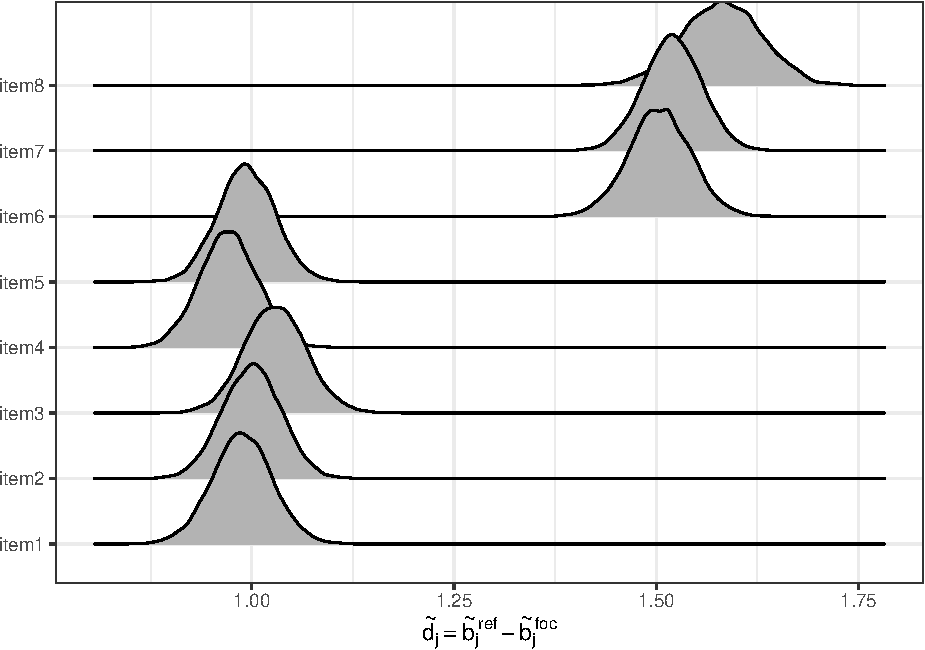
\includegraphics[width=0.7\linewidth]{paper_files/figure-latex/emmilg-1} 

}

\caption{A equal means multiple imputations logit graph (EM-MILG) shows the distribution of how many logits the reference group outperforms the focal group by on each item.}\label{fig:emmilg}
\end{figure}

The same process of using multiple imputations to estimate the distribution of \(\tilde{d_j}\) can be used with a properly identified model. Because the equal means assumption is not made, we refer to the resulting visualization as a multiple imputations logit graph (MILG). As expected, in our demonstration data, selecting the first five items as anchors correctly results in \(\hat d_j \approx 0.5\) for the items with DIF as is shown in the MILG in Figure \ref{fig:milg}.

\begin{figure}[H]

{\centering 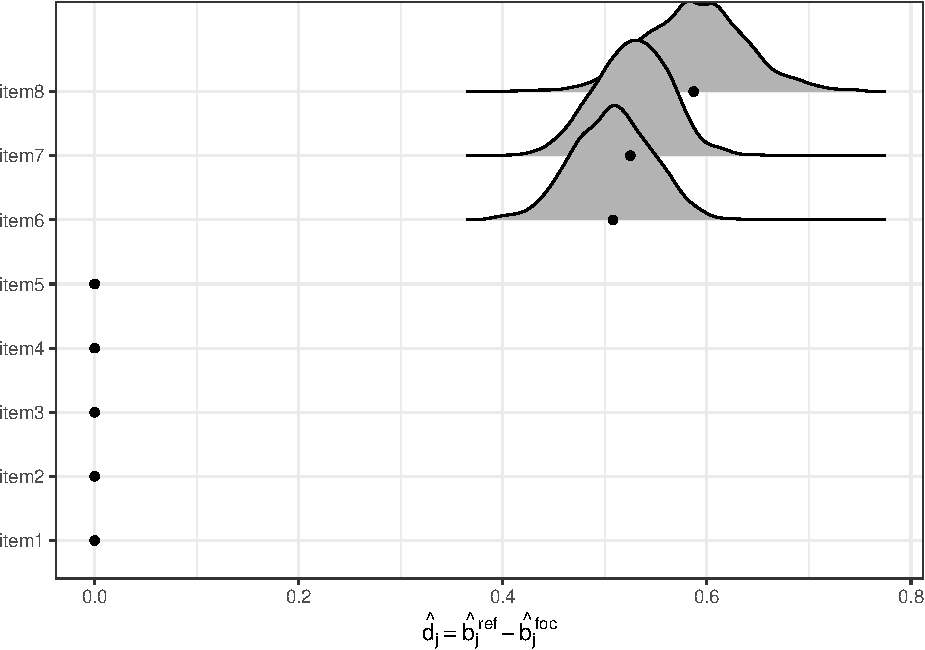
\includegraphics[width=0.7\linewidth]{paper_files/figure-latex/milg-1} 

}

\caption{A multiple imputations logit graph (MILG) shows the distribution of DIF against the focal group. Anchor items are fixed by setting $d_j = 0$.}\label{fig:milg}
\end{figure}

In general, one of our main concerns with traditional AI methods is that they can lull the analyst into a false sense of security: The analyst chooses a method, implements it, and then proceeds as if the method certainly resulted in a model that reflects some objective reality. Our aim with EM-MILG is to combat this concern by presenting all information clearly to the analyst. In the previous example, the analyst may be wary of their results, having seen how arbitrary it was to conclude that the first five and not the last three items are unbiased. Even when other AI methods are used, the analyst can use the EM-MILG as the first step in order to give them a sense of their item response data. And, of course, the MILG can be used to visualize DIF regardless of how the model is identified. We now move on to more traditional AI methods, which don't require judgment from the analyst, but make the majority-of-items-don't-have-DIF assumption more subtly.

\hypertarget{anchoritems}{%
\subsection{Anchor items}\label{anchoritems}}

\hypertarget{all-others-as-anchors-aoaa}{%
\subsubsection{All-others-as-anchors (AOAA)}\label{all-others-as-anchors-aoaa}}

Meade and Wright (\protect\hyperlink{ref-meade2012solving}{2012}) compared the most commonly used AI methods and unequivocally recommended the all-others-as-anchors (AOAA) method. AOAA tests each item for DIF one at a time using all of the other items as anchors. For example, when testing the first item for DIF, all of the other items are used as anchors. This is done using a LRT that compares the baseline model, where all item parameters are fixed across groups, to the flexible model, where the parameters of the tested item are freed across groups (Thissen, Steinberg, and Wainer \protect\hyperlink{ref-thissen1993detection}{1993}). Then, when testing the second item for DIF, once again all of the other items (including the first item) are used as anchors, and so on. The items for which the flexible model outperforms the baseline model (typically based on a \(\chi^2\) test) are identified as having DIF, and the rest of the items become anchor items. AOAA is implemented in the mirt R package, and is called by passing scheme = \enquote{drop} to the DIF function (drop refers to dropping a single constraint when moving from the baseline to the flexible model).

Implicit in the use of AOAA is the assumption that all items not being tested do not exhibit DIF, which is, of course, counter to the underlying rationale for the undertaking. On a practical level, it is thought that AOAA will perform well if a small minority of items have DIF or the DIF is balanced such that some items are biased against the focal group, while others are biased against the reference group. Researchers have noticed the circular logic of AOAA, but have mostly described it indirectly by pointing out inflated Type I errors in simulation studies (Stark, Chernyshenko, and Drasgow \protect\hyperlink{ref-stark2006detecting}{2006}). A simple thought experiment illustrates how AOAA fails: Imagine a three item test with a sufficiently large number of students where the first item has DIF, and the other two do not. Using AOAA, all items test positive for DIF. The last two items incorrectly test positive because including the first item in the anchor set causes the group ability difference to be misestimated. This phenomenon of items with real DIF inducing the appearance of DIF in other items was only indirectly discussed in the literature until Andrich and Hagquist (\protect\hyperlink{ref-andrich2012real}{2012}) coined the term \enquote{artificial DIF}, which is a significant problem in applications of AI methods.

\hypertarget{all-others-as-anchors-all-significant-aoaa-as}{%
\paragraph{All-others-as-anchors-all-significant (AOAA-AS)}\label{all-others-as-anchors-all-significant-aoaa-as}}

One way to attempt to counter artificial DIF is with purification through iterative anchor selection. For example, Drasgow (\protect\hyperlink{ref-drasgow1987study}{1987}) started with AOAA, removed items displaying DIF from the anchor set, then repeated the process iteratively---with items that have been removed from the anchor set allowed to have free parameters across groups in both the baseline and flexible model---until no more items tested positively. Kopf, Zeileis, and Strobl (\protect\hyperlink{ref-kopf2015framework}{2015}) named this technique Iterative-backward-AOAA with \enquote{backward} (as in reverse) referring to beginning with the assumption that all items are DIF-free. We find it clearer to refer to this method as all-others-as-anchors-all-significiant (AOAA-AS). We append \enquote{all-significant} to indicate that all items that test positive for DIF are removed from the anchor set in each iteration. AOAA-AS is implemented in the mirt R package, and is called by passing scheme = \enquote{drop\_sequential} to the DIF function.

We argue that AOAA-AS, while a potential improvement, doesn't solve the fundamental problem of AOAA: What does one do when all items test positive for DIF? With a sufficient sample size and at least one item with DIF, this will necessarily be the case. In our thought experiment, we get the same result with AOAA-AS as we did with AOAA: All items test positive for DIF, and there are no anchor items. Kopf, Zeileis, and Strobl (\protect\hyperlink{ref-kopf2015framework}{2015}) encountered precisely this problem in their simulation study and chose to select a single anchor item randomly. Woods (\protect\hyperlink{ref-woods2009empirical}{2009}) suggested a more straightforward, one-step method: Use AOAA and select the four items that exhibit the least amount of DIF as anchor items.

\hypertarget{all-other-as-anchors-one-at-a-time-aoaa-oat}{%
\paragraph{All-other-as-anchors-one-at-a-time (AOAA-OAT)}\label{all-other-as-anchors-one-at-a-time-aoaa-oat}}

We propose an extension of these methods, all-others-as-anchors-one-at-a-time (AOAA-OAT), which, to our knowledge (and surprise), has not previously been explicitly proposed. AOAA-OAT is inspired by Hagquist and Andrich (\protect\hyperlink{ref-hagquist2017recent}{2017}), who assert that \enquote{items showing DIF initially should not be resolved simultaneously but sequentially} {[}p.~6{]}. Like AOAA-AS, AOAA-OAT starts with AOAA, but only the single item exhibiting the most DIF---based on the \(\chi^2\) test statistic---is removed from the anchor set. The process continues iteratively until no new items display DIF. AOAA-OAT and AOAA-AS are similar in that they are both iterative; the difference is that AOAA-OAT takes the more conservative approach of removing only \emph{one} item in each iteration as opposed to \emph{all} items that test positive for DIF. As a result, we believe that AOAA-OAT is less likely to be \enquote{fooled} by artifical DIF. AOAA-OAT is not currently implemented in the mirt R package.

Applying AOAA-OAT to our thought experiment demonstrates its effectiveness. The initial AOAA removes the real DIF item from the anchor set because it exhibits the most DIF (i.e., because the group difference in performance is most different from the average group difference in performance on the other two items). In the next step, both of the other items test negative for DIF, and we arrive at the correct conclusion.

\hypertarget{equal-means-clustering-emc}{%
\subsubsection{Equal means clustering (EMC)}\label{equal-means-clustering-emc}}

Bechger and Maris (\protect\hyperlink{ref-bechger2015statistical}{2015}) proposed selecting anchor items by identifying clusters of items that function similarly and then choosing one of those clusters to be the \enquote{anchor cluster}. They pointed out that one way around the lack of model identifiability is to consider only relative item parameters. For each group, the relative easinesses for each pair of items can be stored in the (square) matrix \(\mathbf{R}^{\text{ref}}\) with entries \({R_{xy}}^{\text{ref}} = {b_x}^{\text{ref}} - {b_y}^{\text{ref}}\), where \(x\) and \(y\) both index the items. A similar matrix, \(\mathbf{R}^{\text{foc}}\), can be formed. The ultimate matrix of interest is \(\Delta \mathbf{R} \equiv \mathbf{R}^{\text{ref}}-\mathbf{R}^{\text{foc}}\) which is the \enquote{differences between groups in the pairwise differences in (easiness) between items} {[}p.~323{]}.

The general idea of identifying clusters of items is intriguing. However, their approach is complicated, and they did not describe a process for moving from \(\Delta \mathbf{R}\) to an anchor cluster. Pohl, Stets, and Carstensen (\protect\hyperlink{ref-pohl2017cluster}{2017}) extended their work by proposing one such process. They point out that \(\Delta \mathbf{R}\) is skew-symmetric and of rank 1, which means that all information is contained in a single row or column. Accordingly, they recommend k-means clustering on just the first column of \(\Delta \mathbf{R}\) where the number of clusters, k, is chosen by minimizing BIC. They suggest using a combination of cluster size, cluster homogeneity, and cluster parameter precision to choose which of the clusters is the anchor cluster. They conducted a simulation study where some items contained DIF, and, unfortunately, found that BIC identifies only a single cluster, so all items were anchors.

We propose a new cluster-based approach, which we call \enquote{equal means clustering} (EMC). Instead of working with an arbitrary column from \(\Delta \mathbf{R}\), we work with the vector \(\tilde{\mathbf{d}}\), which, as described in the \protect\hyperlink{emmilg}{EM-MILG section}, comes from setting \(\mu^\text{foc} = 0\). Recall that \(\mu^\text{ref}\) is to \(0\) to identify the scale, and thus the name \enquote{equal means clustering}. Instead of choosing k with BIC, we use the gap statistic method recommended by Hastie, Tibshirani, and Walther (\protect\hyperlink{ref-hastie2001estimating}{2001}). Based on the assumption that, at most, a minority of items contain DIF, we choose the largest cluster as the anchor cluster. If there is a tie for the largest cluster, the cluster with the lowest standard deviation of \(\tilde{\mathbf{d}}\) is selected.

\hypertarget{anchor-points}{%
\subsection{Anchor points}\label{anchor-points}}

The previously discussed AI methods identify the model by selecting a set of anchor items that are assumed to be DIF-free. We now discuss the second type of AI methods: The use of an anchor point (Strobl et al. \protect\hyperlink{ref-strobl2018anchor}{2018}). An anchor point directly sets the difference in mean abilities to some value, \(\mu^{\star\text{foc}}\). Anchor point methods have the advantage of not requiring the assumption that any particular item is DIF-free, and, therefore, allowing all items to be tested for DIF. The question then becomes the following: How is the anchor point selected?

\hypertarget{maximizing-the-gini-index-maxgi}{%
\subsubsection{Maximizing the Gini index (MAXGI)}\label{maximizing-the-gini-index-maxgi}}

Strobl et al. (\protect\hyperlink{ref-strobl2018anchor}{2018}) suggest using the Gini index (Gini \protect\hyperlink{ref-gini1912variabilita}{1912}) to select the anchor point. The Gini index is typically used to measure the inequality of wealth distribution in a country. For example, South Africa typically has the highest Gini index of all measured countries, meaning that it is the country with the most unequal wealth distribution (Chitiga, Sekyere, and Tsoanamatsie \protect\hyperlink{ref-chitiga2015income}{2015}). In general, the Gini index \enquote{takes high values if, for example, a small minority of persons has a lot of wealth while the vast majority has very little} (Strobl et al. \protect\hyperlink{ref-strobl2018anchor}{2018}, 7).

Strobl et al. (\protect\hyperlink{ref-strobl2018anchor}{2018}) select \(\mu^{\star\text{foc}}\) by maximizing the Gini index (thus our abbreviation MAXGI). The intuition and assumption is that the anchor point should prioritize the majority of items having little to no DIF and a small subset of items thus having large amounts of DIF. Denoting a function that calculates the Gini index from a vector of non-negative elements as \(G(\mathbf{x})\), MGI sets
\begin{align}
\mu^{\star\text{foc}} = \mathop\mathrm{arg\,max}_{\mu^\text{foc}} G(|\mu^\text{foc} + \tilde{\mathbf{d}}|)
\end{align}
where \(\mu^\text{foc} \in (-\infty, \infty)\) and \(\mu^\text{foc}\) is added to each element of \(\tilde{\mathbf{d}}\).

For the demonstration data, Figure \ref{fig:ginipath} shows the gini index at a variety of possible \(\mu^\text{foc}\) values. The result of MAXGI is \(\mu^{\star\text{foc}} = -0.99\), which is quite close to the data-generating value of -1. Moreover, there is a local maximum at \(\mu^{\text{foc}} \approx 1.5\), which corresponds to the items with DIF. This illustrates that---as Strobl et al. (\protect\hyperlink{ref-strobl2018anchor}{2018}) point out---the search path is informative.

\begin{figure}[H]

{\centering 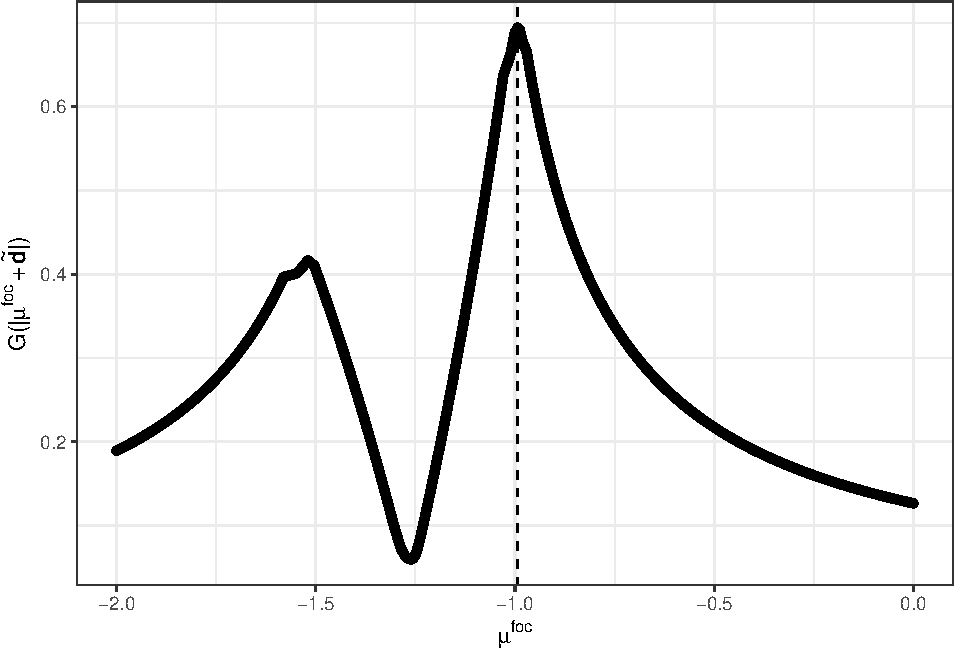
\includegraphics[width=0.7\linewidth]{paper_files/figure-latex/ginipath-1} 

}

\caption{Maximizing the Gini index (MAXGI) to select the anchor point.}\label{fig:ginipath}
\end{figure}

\hypertarget{minimizing-between-curves-minbc}{%
\subsubsection{Minimizing between curves (MINBC)}\label{minimizing-between-curves-minbc}}

Raju's area method (Raju \protect\hyperlink{ref-raju1988area}{1988}) measures the amount of DIF by calculating the area between the item characteristic curves, the function that maps the student's ability to their probability of correct response, of the two groups:
\begin{align}
\text{Area Between Curves} = \int |\text{Pr}(y_j = 1| \theta, b_j^{\text{ref}}) - \text{Pr}(y_j = 1| \theta, b_j^{\text{foc}})|
\end{align}
Raju's area method has been cited as one of the most commonly used IRT-based DIF detection methods (Magis et al. \protect\hyperlink{ref-magis2011generalized}{2011}). However, Raju's area method is not an AI method because the item characteristic curves still need to be linked by anchor items or an anchor point. An additional weakness is that the area is unweighted, so all values of \(\theta\) matter equally, despite some being much more realistic than others.

To adapt Raju's area method into an AI method, we propose a new method, which we call \enquote{minimizing the area between curves} (MINBC). To understand MINBC, imagine a scenario in which the data-generating process is \(\mu^{\text{foc}} = \mu^{\text{ref}}\) and \(d_j = 0 \forall j\), so that the groups have equal ability and there is no DIF. The fundamental identification problem is that there are an infinite number of models with the same likelihood from which to choose. For example, we could correctly assume that the focal group has the same ability as the reference group and fix \(\mu^{\star\text{foc}} = 0\). The model would then estimate \(\hat d_j \approx 0 \forall j\), and we would correctly conclude the groups have the same ability and there is no DIF. Alternatively, we could assume that the focal group has \(\mu^{\star\text{foc}} = 3\). The model would then compensate by finding \(\hat d_j \approx -3 \forall j\), and we would incorrectly conclude that the focal group is high ability, but every item contains DIF against them. Both of these models have the same likelihood, so how should one choose which model to believe? MINBC chooses the model with the least amount of total DIF, as measured by the total weighted area between the item characteristic curves. As a result, the likelihood tie is broken by preferring to explain differences in performance across groups by ability differences (as opposed to DIF).

Denote a function that takes \(\mu^\text{foc}\) as input and estimates \(\hat b_j^\text{foc}\) by fitting a unidimensional Rasch model as \(m_j(\mu^\text{foc})\). The amount of DIF on each item is calculated as
\begin{align}
\text{DIF}_j(\mu^\text{foc}) = \int |\text{Pr}(y_j = 1| \theta, b_j^{\text{ref}}) - \text{Pr}(y_j = 1| \theta, m_j(\mu^\text{foc}))| g(\theta)d\theta
\end{align}
where \(g(\theta)\) is a weighting function such that \(\int g(\theta)d\theta = 1\). The total DIF on the test, then, is
\begin{align}
\text{Total DIF}(\mu^\text{foc}) = \sum_{j} \text{DIF}_j(\mu^\text{foc})
\end{align}
In this way, \(\text{Total DIF}(\mu^\text{foc})\) is a function where the input is \(\mu^\text{foc}\) and the output is the total amount of DIF on the test. MINBC sets
\begin{align}
\mu^{\star\text{foc}} = \mathop\mathrm{arg\,min}_{\mu^\text{foc}} \text{Total DIF}(\mu^\text{foc}).
\end{align}

MINBC is inspired in part by Chalmers, Counsell, and Flora (\protect\hyperlink{ref-chalmers2016might}{2016}), who use the difference between test characteristic curves weighted by \(g(\theta)\) as a measure of differential test functioning (DTF). The selection of \(g(\theta)\) results in the relative weighting of \(\theta\) values. Chalmers, Counsell, and Flora do not discuss how to choose \(g(\theta)\) and in their empirical examples use \(g(\theta)\) uniform for \(-6 \le \theta \le 6\), which may be suboptimal in some cases. It might seem intuitive to choose \(g(\theta) \sim N(0, 1)\) because \(\mu^\text{ref} = 0\), but this choice doesn't take into account the ability distribution of the focal group. If \(\mu^\text{foc} = 3\), wouldn't we also want to prioritize high \(\theta\) values? Accordingly, we set \(g(\theta)\) to be the weighted average of the reference and focal group ability probability density functions:
\begin{align}
g(\theta) = p^\text{ref} \cdot N(\mu^{\text{ref}}, \sigma^{\text{ref}^2}) + (1 - p^\text{ref}) \cdot N(\mu^{\text{foc}}, \sigma^{\text{foc}^2})
\end{align}
where \(p^\text{ref}\) is the proportion of all students that are in the reference group. In this paper, we always have \(p^\text{ref} = 0.5\).

For the demonstration data, Figure \ref{fig:mabc} shows Total DIF at a variety of possible values for \(\mu^\text{foc}\). In this case, MINBC works perfectly and the anchor point is found to be \(\mu^{\star\text{foc}} = -1\). As with MAXGI, the model should then be refit using the identifying assumption that \(\mu^{\text{foc}} = \mu^{\star\text{foc}}\).

\begin{figure}[H]

{\centering 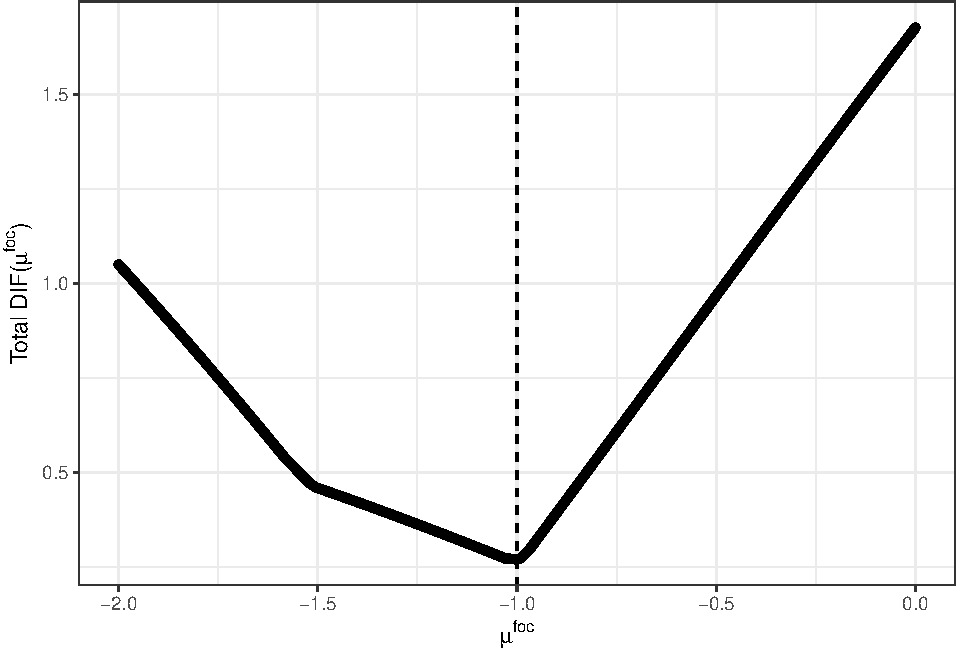
\includegraphics[width=0.7\linewidth]{paper_files/figure-latex/mabc-1} 

}

\caption{Minimizing the area between curves (MINBC) to select the anchor point.}\label{fig:mabc}
\end{figure}

\hypertarget{summary-of-ai-methods}{%
\subsection{Summary of AI methods}\label{summary-of-ai-methods}}

We described a variety of AI methods and their corresponding acronyms. Some of these methods, such as AOAA and EMC, select anchor items, while others, such as MAXGI and MINBC, select an anchor point. Table \ref{table:allmethods} summarizes all of these methods. Figure \ref{fig:allmethodsfig} shows the results for each method on the demonstration data in a MILG.

\begin{table}[H]
\caption{Summary of agnostic identification (AI) methods}
\centering
\begin{tabular}{|p{3cm}|p{4cm}|p{3cm}|p{3cm}|}
\toprule

Method & Description & Literature & Demonstration data \\

\midrule

all-others-as-anchors (AOAA) & Test if each item has DIF by using all of the other items as anchors (not iterative). & Originally proposed by \cite{lord1980} and formalized by \cite{thissen1993detection} & Did not find any anchor items \\\hline

all-others-as-anchors-all-significant (AOAA-AS) & The first iteration is AOAA. All items that test positive for DIF are removed from the anchor set. Continue iterating until no new items test positive for DIF. & Proposed by \cite{drasgow1987study} & Did not find any anchor items \\\hline

all-others-as-anchors-one-at-a-time (AOAA-OAT) & The first iteration is AOAA. Only the item that shows the most extreme DIF is removed from the anchor set. Continue iterating until no new items test positive for DIF. & To our knowledge, not proposed or used previously & Correctly chose the first five items as anchors \\\hline

equal means clustering (EMC) & Cluster items based on differences in performance across groups and choose one of the clusters to be the anchor cluster. & Proposed by \cite{bechger2015statistical} and refined by \cite{pohl2017cluster} & Worked perfectly by finding two clusters of items, one corresponding to the anchor items and the other corresponding to the items with DIF \\\hline

maximizing Gini index (MAXGI) & Arbitrarily set both group means to 0 and then choose an anchor point by maximizing the Gini index & Adapted from work by \cite{strobl2018anchor} & Set $\mu^{\star\text{foc}} = -0.99$, which is quite close to the data generating value of -1 \\\hline

minimizing the area between curves (MINBC) & Of the infinite number of model that maximizes the likelihood of the data, choose the one with the minimum total area between the two groups' item characteristic curves & Built on and inspired by work by \cite{raju1988area} and more recently, \cite{chalmers2016might} & Set $\mu^{\star\text{foc}} = -1$, which is exactly the data generating value\\

\bottomrule
\end{tabular}
\label{table:allmethods}
\end{table}

\begin{figure}[H]

{\centering 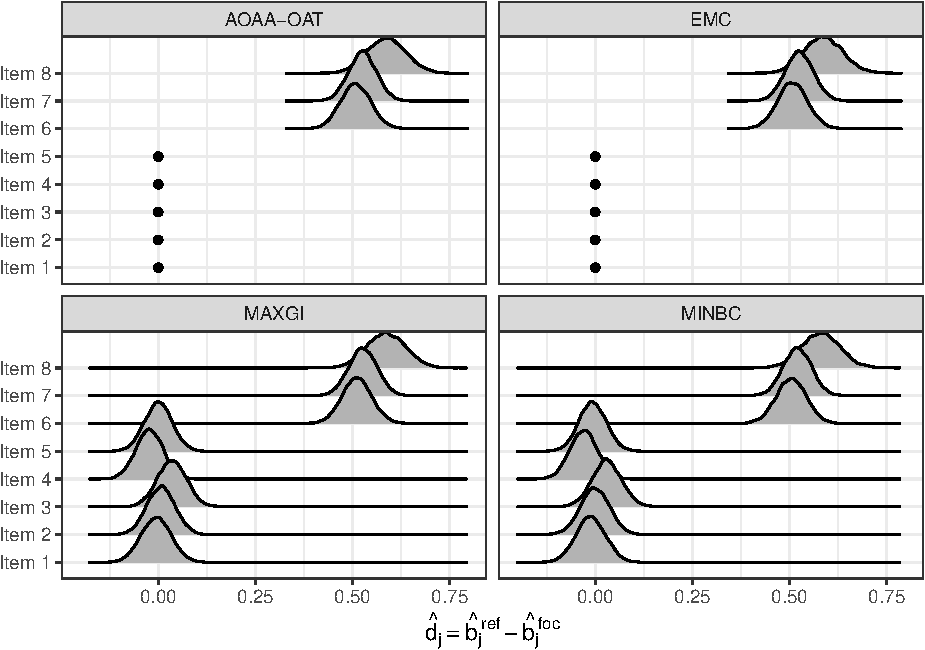
\includegraphics[width=0.7\linewidth]{paper_files/figure-latex/allmethodsfig-1} 

}

\caption{MILG for each of the AI methods applied to the demonstration data. AOAA-OAT and EMC are identified by anchor items (represented by points). MAXGI and MINBC are identified by setting $\mu^{\text{foc}}$ set to the anchor point $\mu^{\star\text{foc}}$. AOAA and AOAA-AS are not included as they did not find an identifying assumption.}\label{fig:allmethodsfig}
\end{figure}

\hypertarget{simstudy}{%
\section{Simulation study}\label{simstudy}}

To compare each of the methods in Table \ref{table:allmethods}, we conducted a simulated study. Our goal was to use a relatively realistic data generating process motivated by the case study in Ackerman (\protect\hyperlink{ref-ackerman1992didactic}{1992}) wherein some items on a math test also depend on a student's verbal ability (the target ability is math ability, and the nuisance ability is verbal ability). Nearly all DIF simulation studies in the literature generate data by simply altering the item easiness parameters for the focal group. As described in \protect\hyperlink{intro}{the introduction}, this setup can be re-written as a two-dimensional compensatory item response model where nuisance ability is the same for all students from the same group. One exception is Walker and Gocer Sahin (\protect\hyperlink{ref-walker2017using}{2017}) who draw each student's target ability and nuisance ability from a two-dimensional normal distribution with varying covariance matrices.

In our simulation study, it was critical that student ability was drawn in a realistic way similar to Walker and Gocer Sahin (\protect\hyperlink{ref-walker2017using}{2017}). However, we don't believe that a compensatory model is realistic in describing a math test where some items depend on verbal ability. For example, it's hard to imagine that a student without the verbal ability to parse a word problem could fully compensate by having a higher math ability. Accordingly, we generated item responses using a simplified version of Sympson's (\protect\hyperlink{ref-sympson1978model}{1978}) noncompensatory item response model in which
\begin{align}
\text{Pr}(y_{ij} = 1 | \theta_i, \eta_i, a_{\eta j}) = \sigma(\theta_i) \cdot \sigma(a_{\eta j}\eta_i)
\end{align}
where, as before, \(\theta_i\) is target ability, \(\eta_i\) is nuisance ability, and \(a_{\eta j}\) is the item's loading on nuisance ability (DeMars \protect\hyperlink{ref-demars2016partially}{2016}).

Computing was done in R (R Core Team \protect\hyperlink{ref-rcore}{2019}), model fitting in the mirt R package (Chalmers \protect\hyperlink{ref-chalmers2012mirt}{2012}), and data wrangling/visualization in the suite of R packages known as the tidyverse (Wickham \protect\hyperlink{ref-tidy}{2017}). Code is available at \emph{(TODO)}.

\hypertarget{drawing-parameters}{%
\subsection{Drawing parameters}\label{drawing-parameters}}

In each run, we simulated 10,000 students with half coming from each of the reference and focal groups. For students from the reference group, target ability and nuisance ability were drawn from the two-dimensional normal distribution with mean {[}\(\mu_\theta^\text{ref} = 0\), \(\mu_\eta^\text{ref} = 0\){]} and covariance matrix \(\begin{bmatrix} 1 & 0.5 \\ 0.5 & 1 \end{bmatrix}\). Abilities for students from the focal group were drawn using the same covariance matrix, but with means {[}\(\mu_\theta^\text{foc} = -0.5\), \(\mu_\eta^\text{foc} = -1\){]}.

The test always has 12 items, but we varied the number of items with DIF from two to six. For items without DIF, \(a_{\eta j} = \infty\) so that the model reduces to \(\text{Pr}(y_{ij} = 1 | \theta_i) = \sigma(\theta_i)\). For items with DIF, \(a_{\eta j}\) is calculated based on Ackerman's (\protect\hyperlink{ref-ackerman1994using}{1994}) angle equation as described in Walker and Gocer Sahin (\protect\hyperlink{ref-walker2017using}{2017}):
\begin{align}
\angle_j = \arccos \dfrac{a_{\theta j}^2}{a_{\theta j}^2 + a_{\eta j}^2}.
\end{align}
An item's angle measures the relative loading of the item on the two dimensions. The lower the angle, the more the item loads on target ability as compared to nuisance ability, which corresponds to less DIF. An angle of 45\(^\circ\) indicates that the item loads equally on the target ability and nuisance ability. Our simple noncompensatory model has \(a_{\theta j} = 1\) for all items so the angle equation reduces to
\begin{align}
\angle_j = \arccos \dfrac{1}{1 + a_{\eta j}^2}.
\end{align}
We are interested in specifying the angle of an item, so the relevant equation becomes
\begin{align}
a_{2j} = \sqrt{\dfrac{1 - \cos(\angle_j)^2}{\cos(\angle_j)^2}}.
\end{align}
For DIF items, we set \(a_{\eta j}\) based on angles with equal intervals between 20\(^\circ\) and 60\(^\circ\). For example, for a test with three DIF items the angles are 20\(^\circ\), 40\(^\circ\), and 60\(^\circ\).

\hypertarget{visualizing-a-run}{%
\subsection{Visualizing a run}\label{visualizing-a-run}}

Figure \ref{fig:difmap} provides intuition about the data generating process by showing the relationship between \(\theta_i\) and \(\text{Pr}(y_{ij} = 1)\) with \(\eta_i\) set to the group mean for a test with six items with DIF. The items are ordered by the amount of DIF such that \(\angle_{j = 7} = 20^\circ\) up to \(\angle_{j = 12} = 60^\circ\).

\begin{figure}[H]

{\centering 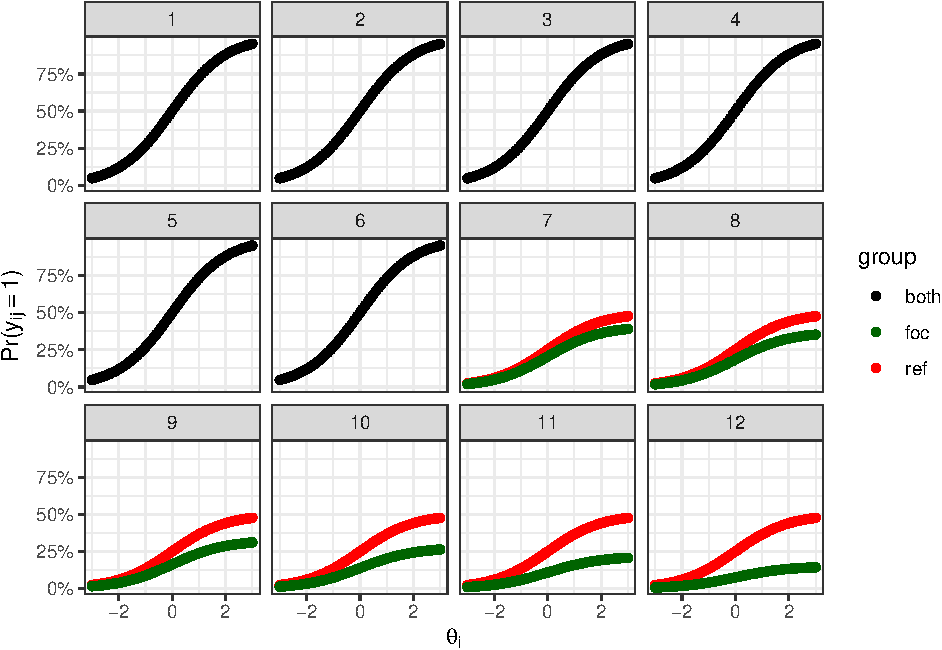
\includegraphics[width=0.7\linewidth]{paper_files/figure-latex/difmap-1} 

}

\caption{For a 12-item test containing 6 items with DIF, the relationship between target ability and probability of correct response with nuisance abilities fixed to the group mean.}\label{fig:difmap}
\end{figure}

Figure \ref{fig:simemmlg} shows the EM-MILG---generated using a Rasch model where both group means are fixed to 0 and item parameters are estimated freely as described in the \protect\hyperlink{anchoritems}{anchor items section}---for one run using the same item parameters that generated Figure \ref{fig:difmap}. As expected, \(\tilde{d_j}\) is about \(\mu_\theta^\text{ref} - \mu_\theta^\text{foc}= 0 - (-0.5) = 0.5\) for the first six items which are DIF free. For the last six items, \(\tilde{d_j}\) increases as \(\angle_j\) increases.

\begin{figure}[H]

{\centering 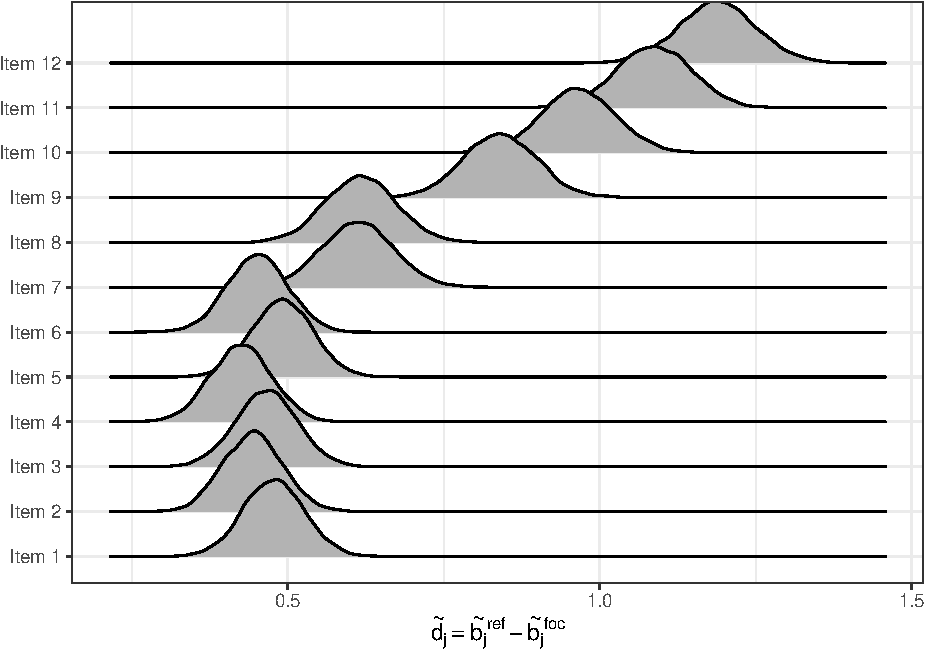
\includegraphics[width=0.7\linewidth]{paper_files/figure-latex/simemmlg-1} 

}

\caption{The EM-MILG for one run using the same item parameters as generated Figure ef{fig:difmap}}\label{fig:simemmlg}
\end{figure}

\hypertarget{outcomes}{%
\subsection{Outcomes}\label{outcomes}}

For each run, we applied each AI method to find the method's identifying assumption. The method's identifying assumption was then used to fit a final model. We compared the performance of those final models according to the following outcomes.

\hypertarget{achievement-gap-residual}{%
\subsubsection{Achievement gap residual}\label{achievement-gap-residual}}

An effective AI method should lead to a final model that accurately estimates the difference between the reference group's mean target ability and the focal group's mean target ability. We refer to this quantity as the achievement gap. Recall that all models set \(\mu_\theta^\text{ref} = 0\), so the achievement gap reduces to \(\mu_\theta^\text{foc}\). The data-generating value of \(\mu_\theta^\text{foc}\) is 0.5, but each run, of course, includes sampling variability. To get at the heart of how well a method is doing, we calculated the achievement gap residual as the method's estimated achievement gap, \(\hat\mu_\theta^\text{foc}\), minus the achievement gap estimated when using only the DIF-free items as anchors. In summary, this outcome measures a method's ability to disentangle differences in target ability from nuisance ability at the group level.

\hypertarget{anchor-items.}{%
\subsubsection{Anchor items.}\label{anchor-items.}}

For the methods that choose a set of anchor items, we looked directly at which anchor items were selected. An effective method should use most of the non-DIF items as anchors (the anchor hit rate) while avoiding using items with DIF as anchors (the false anchor rate).

\hypertarget{results}{%
\subsection{Results}\label{results}}

In total, we executed 100 runs for each of two, three, four, five, and six DIF items. Figure \ref{fig:achievegap} shows each method's performance on the achievement gap residual. AOAA-OAT was the clear winner. It performed nearly perfectly for two, three, or four DIF items. Even when six of the 12 items on the test contained DIF, AOAA-OAT underestimated \(\mu_\theta^\text{foc}\) by only 0.05 standard deviations on its worst run. As expected, artificial DIF caused AOAA and AOAA-AS to begin to exhibit problematic performance as the number of DIF items increased.

EMC performed better than AOAA and AOAA-AS, but worse than the other methods. MINBC and MAXGI performed similarly well with MINBC estimating the achievement gap with more precision but more bias than MAXGI, especially for tests with more than four DIF items. We hypothesize that MINBC's susceptibility to bias results from considering every item. AOAA-OAT, for example, completely disregards an item once it's removed from the anchor set.

\begin{figure}[H]

{\centering 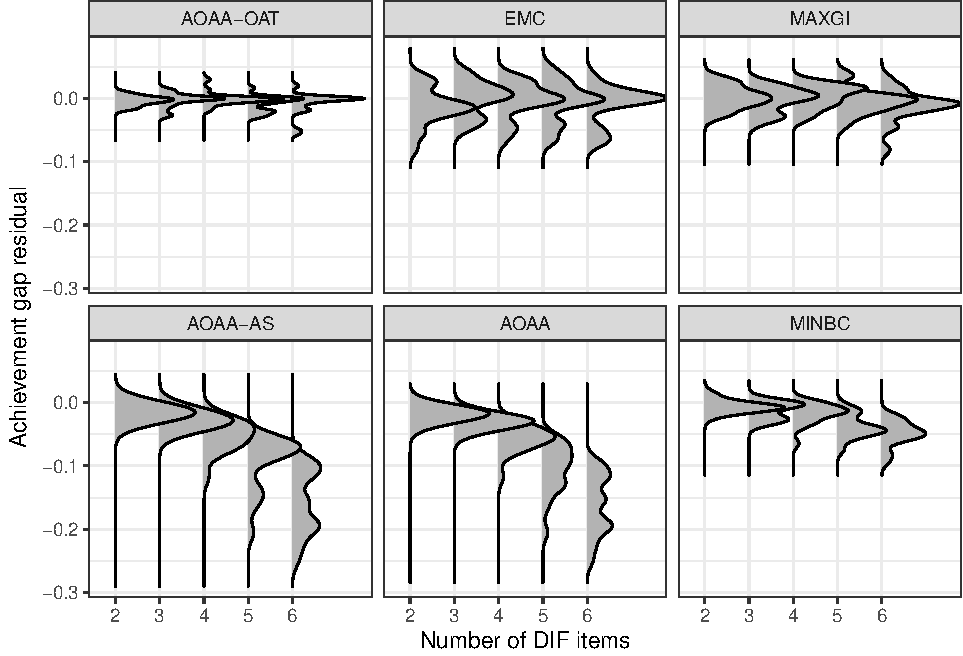
\includegraphics[width=0.7\linewidth]{paper_files/figure-latex/achievegap-1} 

}

\caption{Achievement gap residual distributions across 100 runs for each AI method and number of DIF items.}\label{fig:achievegap}
\end{figure}

Figure \ref{fig:anchorfalse} shows the mean false anchor rates for each method and number of items with DIF. For example, when there were two items with DIF on the test, those two items had \(\angle_{11} = 20^\circ\) and \(\angle_{12} = 60^\circ\). AOAA-OAT never included item 12 in the anchor set, but incorrectly included item 11 in 60 out of the 100 runs. Accordingly, the mean false anchor rate for two DIF items and the AOAA-OAT method was
\begin{align}
\dfrac{\text{Total number of DIF items in the anchor set}}{\text{Number of DIF items on each test} \cdot \text{Number of runs}} = \dfrac{60}{2 \cdot 100} = 30\%.
\end{align}
The fact that the item with 20\(^\circ\) of DIF is most commonly incorrectly included in the anchor set is what drove the counterintuitive result that the mean false anchor rate decreases with more DIF items.

Similarly, Figure \ref{fig:anchorhit} shows the mean anchor hit rates. Remarkably, AOAA-OAT included an average of over \(90\%\) of DIF-free items in the anchor set regardless of the number of DIF items on the test. Interestingly, EMC had a better anchor hit rate on tests with more DIF items. This result appears to be driven by the clustering algorithm sometimes splitting all of the DIF-free items into two separate clusters, especially when most of the items are DIF-free.

\begin{figure}[H]

{\centering 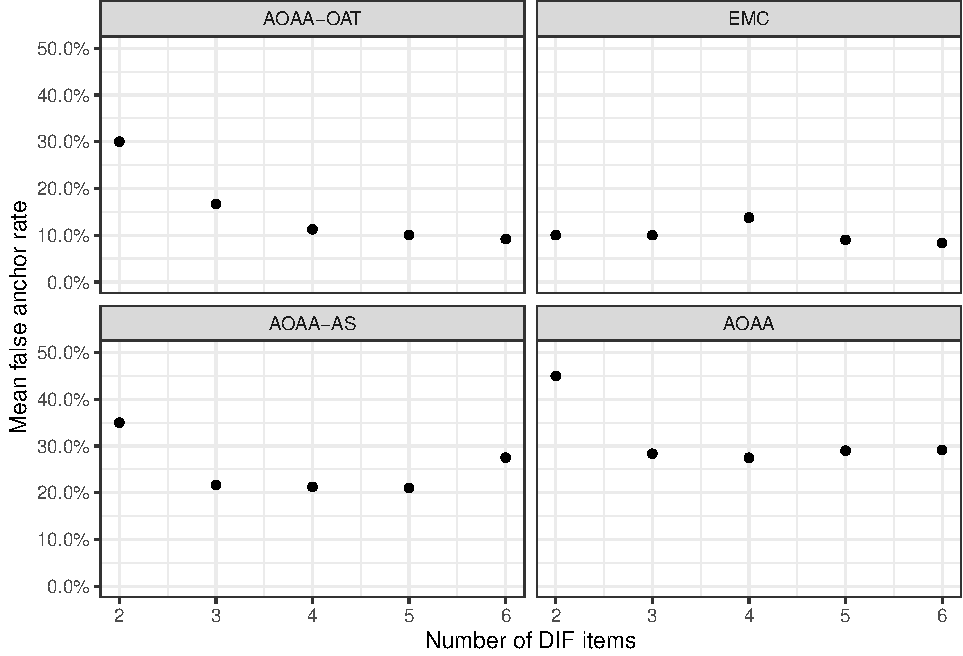
\includegraphics[width=0.7\linewidth]{paper_files/figure-latex/anchorfalse-1} 

}

\caption{Mean false anchor rates across 100 runs for each AI method and number of DIF items.}\label{fig:anchorfalse}
\end{figure}

\begin{figure}[H]

{\centering 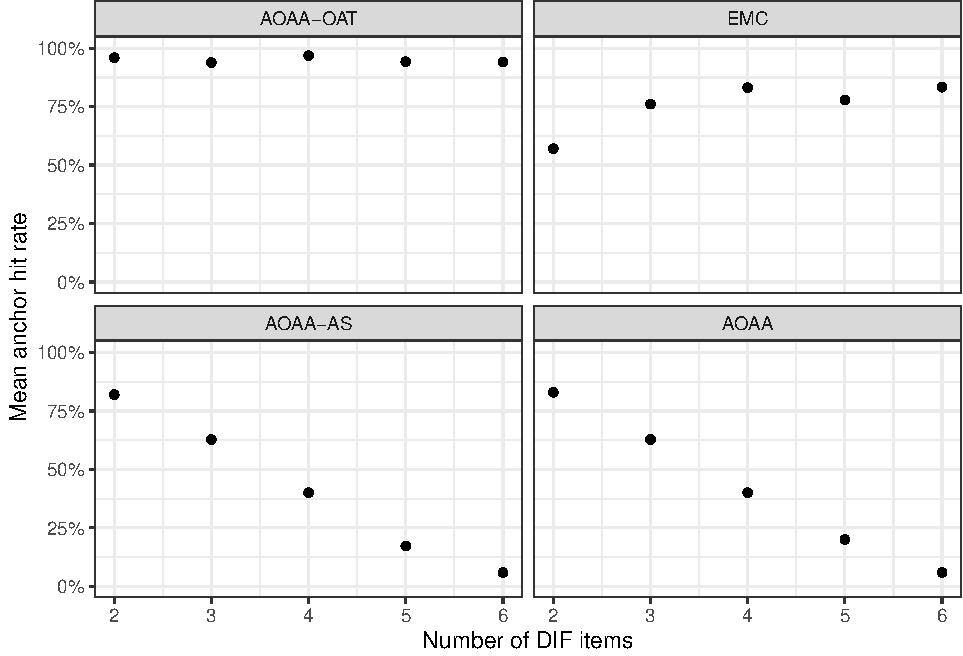
\includegraphics[width=0.7\linewidth]{paper_files/figure-latex/anchorhit-1} 

}

\caption{Mean anchor hit rates across 100 runs for each AI method and number of DIF items.}\label{fig:anchorhit}
\end{figure}

\hypertarget{discussion-and-summary}{%
\section{Discussion and summary}\label{discussion-and-summary}}

Validity hinges on measurement instruments being relatively free of DIF. Such instruments need to be inspected for DIF so that we can be sure of the validity of the conclusions that we draw regardless of the group membership of each student. We reviewed a variety of AI methods, proposed new AI methods, and tested their performance in a simulation study that we believe to be more realistic than the typical DIF simulation study. In particular, we simulated student ability as drawn from a two-dimensional distribution representing a student's target and nuisance ability, and then generated data using a noncompensatory item response model. Our simulation results showed that two of the most common AI methods, AOAA and AOAA-AS, perform quite poorly, especially as the number of items containing DIF grows. This is concerning given both their widespread use and the fact that other methods---AOAA-OAT, EMC, MINGI, and MAXBC---demonstrate superior performance.

AOAA-OAT exhibiting superior performance is an important finding given that it is, to our knowledge, not used currently. We advocate for its widespread use. One drawback of the AOAA-OAT method is that it is computationally expensive. For example, finding three items containing DIF on a 12-item test requires fitting 46 item response models, and that number grows as either the test length or the number of items testing positive for DIF grows. However, we believe the computational costs are worthwhile given the performance of this method relative to more widely implemented alternatives. To increase AOAA-OAT's use, we recommend its implementation (perhaps as the default) in popular IRT software such as the mirt R package.

In addition to exploring and testing algorithmic AI methods, we introduced a method, the EM-MILG, that an analyst can use to visualize the amount of potential DIF in their data. This method can be used either to build their intuition or as a way in which they can select anchor items by hand. The EM-MILG's sibling method, the MILG, is, we believe, the best way to visualize the results of a DIF analysis after anchor items have been selected.

We emphasize that the EM-MILG gives a clear view of the possibility of DIF on a test. For example, in Figure \ref{fig:simemmlg} it's clear that the gap between focal and reference group performance across items on the test varies greatly. By assuming that the majority of items do not contain DIF, AI methods essentially make an educated guess about the relative responsibility of group ability differences vs.~DIF. Our simulation focused on a scenario wherein half of the items are DIF-free and the other half have escalating amounts of DIF. Different patterns of DIF (as visualized in an EM-MILG) will pose different challenges.

For example, imagine a test in which the focal group outperforms the reference group by one logit on half of the items, and the reference group outperforms the focal group by one logit on the other half of the items. What should an AI method conclude in this case? AOAA and AOAA-AS will likely (perhaps rightfully) fail to find any anchor items; MINBC will choose an anchor point close to zero (and will find DIF in all items); MAXGI will arbitrarily choose an anchor point within one of the groups of items (and will find DIF in the other group of items); and AOAA-OAT and EMC will arbitrarily choose one of the groups of items to be anchor items (and, like MAXGI, will find DIF in the other group of items). This example illustrates that some patterns of DIF are such that the analyst should probably remain agnostic. In these cases, we suggest that the analyst report the nature of potential DIF using a EM-MILG. Future work might produce methods for quantifying what is visualized in a EM-MILG, essentially making a metric for the amount of potential DIF on a test.

Moreover, future work should test these methods' performance under a greater variety of data generating conditions. For example, changing the compensatory nature of the data generating model or adding additional nuisance ability dimensions. Finally, our work focused on the Rasch model, and it is of great interest to consider how these methods extend and perform when the goal is to detect and correct for DIF when fitting other types of item response models.

\clearpage

\bibliographystyle{apa}
\bibliography{paper.bib}

\hypertarget{refs}{}
\leavevmode\hypertarget{ref-ackerman1992didactic}{}%
Ackerman, Terry A. 1992. ``A Didactic Explanation of Item Bias, Item Impact, and Item Validity from a Multidimensional Perspective.'' \emph{Journal of Educational Measurement} 29 (1): 67--91.

\leavevmode\hypertarget{ref-ackerman1994using}{}%
---------. 1994. ``Using Multidimensional Item Response Theory to Understand What Items and Tests Are Measuring.'' \emph{Applied Measurement in Education} 7 (4): 255--78.

\leavevmode\hypertarget{ref-andrich2012real}{}%
Andrich, David, and Curt Hagquist. 2012. ``Real and Artificial Differential Item Functioning.'' \emph{Journal of Educational and Behavioral Statistics} 37 (3): 387--416.

\leavevmode\hypertarget{ref-bechger2015statistical}{}%
Bechger, Timo M, and Gunter Maris. 2015. ``A Statistical Test for Differential Item Pair Functioning.'' \emph{Psychometrika} 80 (2): 317--40.

\leavevmode\hypertarget{ref-bock1981marginal}{}%
Bock, R Darrell, and Murray Aitkin. 1981. ``Marginal Maximum Likelihood Estimation of Item Parameters: Application of an Em Algorithm.'' \emph{Psychometrika} 46 (4): 443--59.

\leavevmode\hypertarget{ref-camilli1992conceptual}{}%
Camilli, Gregory. 1992. ``A Conceptual Analysis of Differential Item Functioning in Terms of a Multidimensional Item Response Model.'' \emph{Applied Psychological Measurement} 16 (2): 129--47.

\leavevmode\hypertarget{ref-chalmers2012mirt}{}%
Chalmers, R Philip. 2012. ``Mirt: A Multidimensional Item Response Theory Package for the R Environment.'' \emph{Journal of Statistical Software} 48 (6): 1--29.

\leavevmode\hypertarget{ref-chalmers2018numerical}{}%
---------. 2018. ``Numerical Approximation of the Observed Information Matrix with Oakes' Identity.'' \emph{British Journal of Mathematical and Statistical Psychology} 71 (3): 415--36.

\leavevmode\hypertarget{ref-chalmers2016might}{}%
Chalmers, R Philip, Alyssa Counsell, and David B Flora. 2016. ``It Might Not Make a Big Dif: Improved Differential Test Functioning Statistics That Account for Sampling Variability.'' \emph{Educational and Psychological Measurement} 76 (1): 114--40.

\leavevmode\hypertarget{ref-chitiga2015income}{}%
Chitiga, Margaret, E Sekyere, and N Tsoanamatsie. 2015. ``Income Inequality and Limitations of the Gini Index: The Case of South Africa.'' \emph{Human Sciences Research Council (HSRC), Available at: Http://Www. Hsrc. Ac. Za/En/Review/Hsrc-Review-November-2014/Limitations-of-Gini-Index, Site Accessed} 2.

\leavevmode\hypertarget{ref-cook1987problems}{}%
Cook, Linda L, and Nancy S Paterson. 1987. ``Problems Related to the Use of Conventional and Item Response Theory Equating Methods in Less Than Optimal Circumstances.'' \emph{Applied Psychological Measurement} 11 (3): 225--44.

\leavevmode\hypertarget{ref-demars2016partially}{}%
DeMars, Christine E. 2016. ``Partially Compensatory Multidimensional Item Response Theory Models: Two Alternate Model Forms.'' \emph{Educational and Psychological Measurement} 76 (2): 231--57.

\leavevmode\hypertarget{ref-drasgow1987study}{}%
Drasgow, Fritz. 1987. ``Study of the Measurement Bias of Two Standardized Psychological Tests.'' \emph{Journal of Applied Psychology} 72 (1): 19.

\leavevmode\hypertarget{ref-furlow2009impact}{}%
Furlow, Carolyn F, Terris Raiford Ross, and Phill Gagné. 2009. ``The Impact of Multidimensionality on the Detection of Differential Bundle Functioning Using Simultaneous Item Bias Test.'' \emph{Applied Psychological Measurement} 33 (6): 441--64.

\leavevmode\hypertarget{ref-gini1912variabilita}{}%
Gini, Corrado. 1912. ``Variabilità E Mutabilità (Variability and Mutability).'' \emph{Tipografia Di Paolo Cuppini, Bologna, Italy}, 156.

\leavevmode\hypertarget{ref-hagquist2017recent}{}%
Hagquist, Curt, and David Andrich. 2017. ``Recent Advances in Analysis of Differential Item Functioning in Health Research Using the Rasch Model.'' \emph{Health and Quality of Life Outcomes} 15 (1): 181.

\leavevmode\hypertarget{ref-hastie2001estimating}{}%
Hastie, Trevor, Robert Tibshirani, and Guenther Walther. 2001. ``Estimating the Number of Data Clusters via the Gap Statistic.'' \emph{J Roy Stat Soc B} 63: 411--23.

\leavevmode\hypertarget{ref-holland1986differential}{}%
Holland, Paul W, and Dorothy T Thayer. 1986. ``Differential Item Functioning and the Mantel-Haenszel Procedure.'' \emph{ETS Research Report Series} 1986 (2): i--24.

\leavevmode\hypertarget{ref-kirisci2001robustness}{}%
Kirisci, Levent, Tse-chi Hsu, and Lifa Yu. 2001. ``Robustness of Item Parameter Estimation Programs to Assumptions of Unidimensionality and Normality.'' \emph{Applied Psychological Measurement} 25 (2): 146--62.

\leavevmode\hypertarget{ref-kopf2015framework}{}%
Kopf, Julia, Achim Zeileis, and Carolin Strobl. 2015. ``A Framework for Anchor Methods and an Iterative Forward Approach for Dif Detection.'' \emph{Applied Psychological Measurement} 39 (2): 83--103.

\leavevmode\hypertarget{ref-magis2011generalized}{}%
Magis, David, Gilles Raı̂che, Sébastien Béland, and Paul Gérard. 2011. ``A Generalized Logistic Regression Procedure to Detect Differential Item Functioning Among Multiple Groups.'' \emph{International Journal of Testing} 11 (4): 365--86.

\leavevmode\hypertarget{ref-meade2012solving}{}%
Meade, Adam W, and Natalie A Wright. 2012. ``Solving the Measurement Invariance Anchor Item Problem in Item Response Theory.'' \emph{Journal of Applied Psychology} 97 (5): 1016.

\leavevmode\hypertarget{ref-pohl2017cluster}{}%
Pohl, Steffi, Eric Stets, and Claus H Carstensen. 2017. ``Cluster-Based Anchor Item Identification and Selection.''

\leavevmode\hypertarget{ref-raju1988area}{}%
Raju, Nambury S. 1988. ``The Area Between Two Item Characteristic Curves.'' \emph{Psychometrika} 53 (4): 495--502.

\leavevmode\hypertarget{ref-rcore}{}%
R Core Team. 2019. \emph{R: A Language and Environment for Statistical Computing}. Vienna, Austria: R Foundation for Statistical Computing. \url{https://www.R-project.org/}.

\leavevmode\hypertarget{ref-stark2006detecting}{}%
Stark, Stephen, Oleksandr S Chernyshenko, and Fritz Drasgow. 2006. ``Detecting Differential Item Functioning with Confirmatory Factor Analysis and Item Response Theory: Toward a Unified Strategy.'' \emph{Journal of Applied Psychology} 91 (6): 1292.

\leavevmode\hypertarget{ref-strobl2018anchor}{}%
Strobl, Carolin, Julia Kopf, Raphael Hartmann, and Achim Zeileis. 2018. ``Anchor Point Selection: An Approach for Anchoring Without Anchor Items.'' Working Papers in Economics; Statistics.

\leavevmode\hypertarget{ref-swaminathan1990detecting}{}%
Swaminathan, Hariharan, and H Jane Rogers. 1990. ``Detecting Differential Item Functioning Using Logistic Regression Procedures.'' \emph{Journal of Educational Measurement} 27 (4): 361--70.

\leavevmode\hypertarget{ref-sympson1978model}{}%
Sympson, James B. 1978. ``A Model for Testing with Multidimensional Items.'' In \emph{Proceedings of the 1977 Computerized Adaptive Testing Conference}. 00014.

\leavevmode\hypertarget{ref-talbot2013taking}{}%
Talbot III, Robert M. 2013. ``Taking an Item-Level Approach to Measuring Change with the Force and Motion Conceptual Evaluation: An Application of Item Response Theory.'' \emph{School Science and Mathematics} 113 (7): 356--65.

\leavevmode\hypertarget{ref-thissen1986taxonomy}{}%
Thissen, David, and Lynne Steinberg. 1986. ``A Taxonomy of Item Response Models.'' \emph{Psychometrika} 51 (4): 567--77.

\leavevmode\hypertarget{ref-thissen1993detection}{}%
Thissen, David, Lynne Steinberg, and Howard Wainer. 1993. ``Detection of Differential Item Functioning Using the Parameters of Item Response Models.''

\leavevmode\hypertarget{ref-topczewski2013comparison}{}%
Topczewski, Anna, Zhongmin Cui, David Woodruff, Hanwei Chen, and Yu Fang. 2013. ``A Comparison of Four Linear Equating Methods for the Common-Item Nonequivalent Groups Design Using Simulation Methods. ACT Research Report Series, 2013 (2).'' \emph{ACT, Inc.}

\leavevmode\hypertarget{ref-walker2017using}{}%
Walker, Cindy M, and Sakine Gocer Sahin. 2017. ``Using a Multidimensional Irt Framework to Better Understand Differential Item Functioning (Dif): A Tale of Three Dif Detection Procedures.'' \emph{Educational and Psychological Measurement} 77 (6): 945--70.

\leavevmode\hypertarget{ref-wang2012dif}{}%
Wang, Wen-Chung, Ching-Lin Shih, and Guo-Wei Sun. 2012. ``The Dif-Free-Then-Dif Strategy for the Assessment of Differential Item Functioning.'' \emph{Educational and Psychological Measurement} 72 (4): 687--708.

\leavevmode\hypertarget{ref-tidy}{}%
Wickham, Hadley. 2017. \emph{Tidyverse: Easily Install and Load the 'Tidyverse'}. \url{https://CRAN.R-project.org/package=tidyverse}.

\leavevmode\hypertarget{ref-woods2009empirical}{}%
Woods, Carol M. 2009. ``Empirical Selection of Anchors for Tests of Differential Item Functioning.'' \emph{Applied Psychological Measurement} 33 (1): 42--57.

\leavevmode\hypertarget{ref-yang2012characterizing}{}%
Yang, Ji Seung, Mark Hansen, and Li Cai. 2012. ``Characterizing Sources of Uncertainty in Item Response Theory Scale Scores.'' \emph{Educational and Psychological Measurement} 72 (2): 264--90.

\end{document}
